% \iffalse
\let\negmedspace\undefined
\let\negthickspace\undefined
\documentclass[journal,12pt,twocolumn]{IEEEtran}
\usepackage{cite}
\usepackage{amsmath,amssymb,amsfonts,amsthm}
\usepackage{algorithmic}
\usepackage{graphicx}
\usepackage{textcomp}
\usepackage{xcolor}
\usepackage{txfonts}
\usepackage{listings}
\usepackage{enumitem}
\usepackage{mathtools}
\usepackage{gensymb}
\usepackage{comment}
\usepackage[breaklinks=true]{hyperref}
\usepackage{tkz-euclide} 
\usepackage{tikz}
\usepackage{circuitikz}
\usepackage{listings}
\usepackage{gvv}                                        
\def\inputGnumericTable{}                                 
\usepackage[latin1]{inputenc}                                
\usepackage{color}                                            
\usepackage{array}                                            
\usepackage{longtable}                                       
\usepackage{calc}                                             
\usepackage{multirow}                                         
\usepackage{hhline}                                           
\usepackage{ifthen}                                           
\usepackage{lscape}
\usepackage{caption}
\newtheorem{theorem}{Theorem}[section]
\newtheorem{problem}{Problem}
\newtheorem{proposition}{Proposition}[section]
\newtheorem{lemma}{Lemma}[section]
\newtheorem{corollary}[theorem]{Corollary}
\newtheorem{example}{Example}[section]
\newtheorem{definition}[problem]{Definition}
\newcommand{\BEQA}{\begin{eqnarray}}
\newcommand{\EEQA}{\end{eqnarray}}
\newcommand{\define}{\stackrel{\triangle}{=}}
\theoremstyle{remark}
\newtheorem{rem}{Remark}
\begin{document}
\parindent 0px
\bibliographystyle{IEEEtran}
\vspace{3cm}

\title{GATE 2021 1.CH}
\author{EE23BTECH11012 - Chavan Dinesh$^{*}$% <-this % stops a space
}
\maketitle
\newpage
\bigskip

\renewcommand{\thefigure}{\arabic{figure}}
\renewcommand{\thetable}{\arabic{table}}
\large\textbf{\textsl{Question:}}
An ordinary differential equation (ODE) $\frac{dy}{dx} = 2y$ with an initial condition $y(0) = 1$ has the analytical
solution $y = e^{2x}$
 Using Runge-Kutta second order method, numerically integrate the ODE to calculate $y$ at $x = 0.5$ using a
step size of $h = 0.5$.
 If the relative percentage error is defined as 
 \begin{align}
 \epsilon = \left|\frac{y_{analytical} - y_{numerical}}{y_{analytical}}\right| \times 100 \nonumber
 \end{align}
 then the value of $\epsilon$ at $x = 0.5$ is
 
\hfill(GATE 1 CH 2021)

\solution

\begin{table}[htbp]
    \centering
    \begin{tabular}{|c|c|c|}
\hline
   \textbf{Parameter}  & \textbf{Description} & \textbf{Value}\\
   \hline
   R   & Resistance & $10 \omega$\\
   \hline
  C & Capacitance & $100 \micro F$ \\
  \hline
  L & Inductor & $50mH$\\
  \hline
  Z & Impedance & \\
  \hline
  $Z_{new}$ &New Impedance & \\
  \hline
\end{tabular}

    \caption{}
    \label{tab:input_parameters.33.BM.2022}
\end{table}

% \begin{figure}[!ht]
%     \centering
%         \begin{circuitikz}
    \draw(0, 0) -- (1, 0);
    \draw(1, 0) to [L, l = $50\text{mH}$](2, 0);
    \draw(2, 0) -- (3, 0);
    \draw(3, 0) to [C, l = $100\, \mu\text{F}$](4, 0);
    \draw(4, 0) -- (5, 0);
    \draw(5, 0) to [R, l = $10\Omega$](6, 0);
    \draw(0, 0) -- (0, -2);
    \draw[->] (0, -1) node[left] {$I(t)$} -- (0, -1);
    \draw(6, 0) -- (7, 0);
    \draw(7, 0) -- (7, -2);
    \draw(0, -2) -- (3, -2);
    \draw(7, -2) -- (7, -2);
    \draw(3, -2) to [sV, l = $V(t)$](4, -2);
    \draw(4, -2) -- (7, -2);
\end{circuitikz}

%     \caption{}
%     \label{fig:fig1.33.BM.2022}
% \end{figure}

Analytical solution is given by:
\begin{align}
    y = e^{2x}
\end{align}
At $x = 0.5$, analytical solution is 
\begin{align}
    y(0.5) = e^{2\times 0.5} = 2.718 
\end{align}
According to question:
\begin{align}
    f(x,y) = \frac{dy}{dx} = 2y
\end{align}
By Runge-kutta $2^{nd}$ order method, 
\begin{align}
    K_1 = hf(x_o,y_o) = h(2y_o)\\
    K_1 = 0.5(2 \times 1) = 1
\end{align}
\begin{align}
    K_2 = h[f(x_o + h, y_o + K_1)]\\
    K_2 = h[2(1 +1)]\\
    K_2 = 0.5 \times 4 = 2 
\end{align}
\begin{align}
    K = \frac{K_1 + K_2}{2} = \frac{1 +2}{2} = 1.5
\end{align}
\begin{align}
    y_{_{1}} = y_{numerical} = y_o + K = 1 + 1.5 = 2.5 
\end{align}
Hence, 
\begin{align}
    \epsilon = \left|\frac{2.718 - 2.5}{2.718}\right| \times 100 \\
    \epsilon = \frac{0.218}{2.718}\times 100 = 8\%
 \end{align}
% \begin{figure}[ht]
%     \centering
%     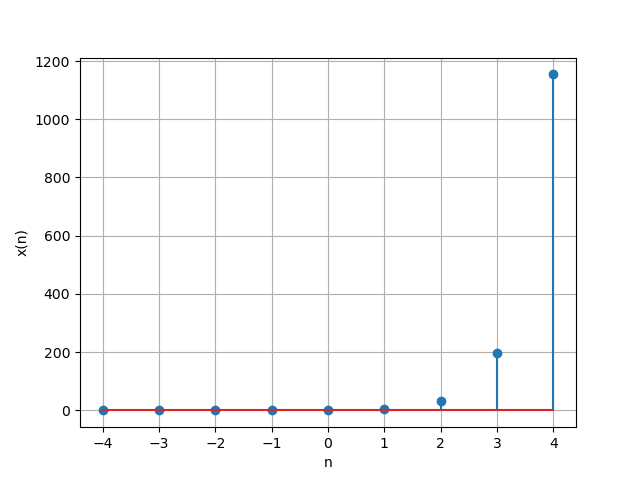
\includegraphics[width = \columnwidth]{figs/x_n_stem_plot.png}
%     \caption{}
%     \label{fig:graph1.11.9.3.28}
% \end{figure}

\bibliographystyle{IEEEtran}
\end{document}
